% !TeX TS-program = xelatex

\documentclass{resume}
\ResumeName{陈子渝}

\usepackage{graphicx}
\usepackage{tikz}
\usepackage{fontawesome5}

% 个人主页地址（自定义域名，托管于 GitHub Pages），如更换只需改这一处
\newcommand{\MyHomepage}{ziyuchen.me}

% 中文标点半角压缩，避免引号等标点占满全角留白过大
\xeCJKsetup{PunctStyle=banjiao}

\linespread{1.05}

\begin{document}

\ResumeContacts{
  硕士,%
  18582894157,%
  \ResumeUrl{mailto:chenziyu089@163.com}{chenziyu089@163.com},%
  \faHome~\ResumeUrl{https://\MyHomepage}{\MyHomepage}%
}

% 证件照：绝对定位于页面右上角，不占据正文流高度
\begin{tikzpicture}[remember picture, overlay]
  \node[anchor=north east, xshift=-0.65cm, yshift=-0.55cm]
    at (current page.north east)
    {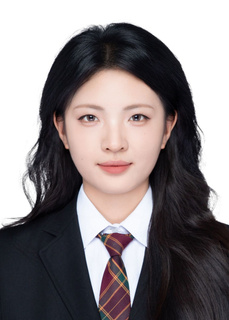
\includegraphics[width=2.0cm]{photo.jpg}};
\end{tikzpicture}%

\ResumeTitle

\section{教育背景}

\ResumeItem
[电子科技大学|硕士研究生]
{电子科技大学}
[\textnormal{经济管理|} 硕士]
[2024.09—2027.07]

\begin{itemize}
  \item \textbf{荣誉奖励：} 院级一等奖学金、院级二等奖学金；硕士入学考试专业第一（跨专业考研）
  \item \textbf{主修课程：} 管理信息系统、数据与算法治理，主要研究方向为数据治理
  \item \textbf{研究成果：} 论文被 \textbf{EMNLP 2026} 录用（NLP 顶会）：\textit{FedLing: Linguistic-Structure-Aware Federated Learning for Fair Multilingual LLM Adaptation}
\end{itemize}

\ResumeItem
[上海师范大学|本科生]
{上海师范大学}
[\textnormal{旅游管理|} 本科]
[2020.09—2024.07]

\begin{itemize}
  \item \textbf{荣誉奖励：} 校级奖学金一次、院级奖学金两次、上海市“星光计划”技能大赛个人一等奖
  \item \textbf{主修课程：} 管理学、市场营销、微观经济学、宏观经济学
\end{itemize}

\section{实习经历}

\ResumeItem
[携程（上海总部）|产品运营实习生]
{携程（上海总部）}
[\textnormal{海外业务部 | 产品运营实习生}]
[2024.05—2024.09]

\begin{itemize}

\item \textbf{Google 渠道产品能力建设。} 对接 Google 平台业务、内部产品及研发团队，梳理外部平台规则与业务场景，将需求拆解为功能范围、字段口径、展示规则和验收项；协同推动“多日通票类型支持”“Google Discover 景点内容接入”2 项需求按期上线，上线后相关景点内容曝光量提升 \textbf{11\%}。

\item \textbf{渠道漏斗分析与产品迭代。} 基于 Google Trends、Google Search Console 及业务数据，按区域、目的地和景点跟踪搜索热度、曝光及转化表现，周度复盘、月度识别 \textbf{3+} 个异常或增长机会；据此提出实时空位查询、组合票务和多语种客服等方案，推动 2 项进入需求调研，页面优化后目标页面转化率提升约 \textbf{6\%}。

\item \textbf{跨平台数据治理。} 针对 Google 平台与内部系统字段口径不一致问题，梳理名称、价格、库存和退改政策等 \textbf{20+} 个关键字段的映射与核验规则，完成东京迪士尼、罗马斗兽场等 \textbf{55 个}高潜景点的首次接入；月均交付 \textbf{30+} 项挂接与优化任务，上线批次无重大数据错误，相关页面跳出率下降 \textbf{6\%}，渠道整体转化率提升 \textbf{3\%}。

\item \textbf{异常治理与问题闭环。} 归类库存更新、接口异常和确认信息缺失等高频问题，依据影响范围与紧急程度分级，执行 2 小时响应、8 小时初步方案的处理标准；累计协同产品、研发及供应商闭环 \textbf{60+ 个}问题，均在 \textbf{12 小时}内完成处理，并将重复问题沉淀为数据规则或产品优化项。

\end{itemize}

\ResumeItem
[成都中国国际旅行社|市场部实习生]
{成都中国国际旅行社}
[\textnormal{市场部实习生}]
[2023.09—2024.02]

\begin{itemize}

\item \textbf{社群增长与活动运营。} 围绕新产品冷启动及社群新增目标，策划朋友圈传播、红包雨等线上活动，并按“内容触达—用户入群—业务咨询”漏斗复盘效果；累计触达 \textbf{15,000+ 人次}，带来 \textbf{200+ 次}咨询，首日新增用户 \textbf{235 人}，目标达成率 \textbf{117\%}，推动社群规模 3 个月内增长近 \textbf{1.4 万人}。

\item \textbf{用户需求分析与订单转化。} 基于出行时间、预算、目的地和同行人群等信息进行用户需求分层，完成产品匹配、方案沟通及后续跟进，实习期间独立完成 \textbf{16 单}定制旅行订单转化。

\end{itemize}

\section[校园经历]{校园经历}

\begin{itemize}
  \item \textbf{校研究生会干事（获评校级“研究生优秀干事”）：} 负责“第十七届研究生青春风采大赛”“庆祖国 75 周年华诞环校跑”等活动设计与筹办，协助完成 4 项校级活动落地，服务研究生群体 2,000 余人
  \item \textbf{学生会主席团成员（本科）：} 负责文体活动的组织协调与运营，统筹“校级文化交流月”“社团文化节”等 7 场校级活动，覆盖师生 5,000 余人
  \item \textbf{班级团支书（本科，4 年）：} 负责团支部建设与青年思想引领，组织主题团日活动 13 场、理论学习 17 次，覆盖班级全体成员
\end{itemize}

\section[技术能力]{技术能力}

\begin{itemize}
  \item \textbf{数据分析：} SQL、Python（Pandas）、Excel、Google Analytics、Google Trends、Google Search Console
  \item \textbf{产品设计：} Axure、Figma、墨刀、蓝湖、XMind、PS；可独立完成需求分析、流程设计、原型及需求文档
  \item \textbf{产品方法：} 竞品分析、用户画像、A/B 测试、数据驱动迭代
  \item \textbf{项目协作：} JIRA、Confluence、TAPD、飞书、敏捷开发（Agile/Scrum）；具备产品、研发、运营及外部平台多方协作经验
  \item \textbf{AI 应用：} 熟练使用 Claude Code、Codex 等 AI Agent 工具辅助需求分析、原型验证与数据处理
  \item \textbf{语言能力：} CET-6
  \item \textbf{证书：} 上海市计算机一级证书、全国导游资格证书、携程旅游定制师证、普通话二级甲等证书、志愿者证
\end{itemize}

\section[个人总结]{个人总结}

\begin{itemize}
  \item \textbf{数据驱动：} 以数据定位问题、验证效果，实习期间以数据监测驱动优化，推动曝光量提升 11\%、转化率提升 6\%
  \item \textbf{协调沟通：} 擅长跨部门沟通协调，实习期间独立对接 60+ 业务方，调动内外部资源推动需求落地
  \item \textbf{学习/抗压能力：} 跨专业考研专业第一，能快速理解高复杂度的产品与算法逻辑，同时推进多个重点项目
  \item \textbf{商业 Sense：} 管理学背景出身，兼具管理视角与互联网商业变现知识，擅长用户洞察与需求匹配
  \item \textbf{求职意向：} 产品经理 / 产品运营（2027 届硕士，实习与校招岗位均可，有海外业务或 AI 产品方向更佳）
\end{itemize}

\end{document}
